\documentclass[10pt]{article}

% a4large.sty -- fill an A4 (210mm x 297mm) page
% Note: 1 inch = 25.4 mm = 72.27 pt
%       1 pt   =  3.5 mm (approx)

\usepackage[paperheight=297mm,
            paperwidth=210mm,
            tmargin=28mm, 
            headheight=0mm, 
            headsep=0mm,
            textheight=240mm,
            footskip=7mm,
            textwidth=159.2mm,
            bindingoffset=10mm,
            twoside
            ]{geometry}

% paragraph setup
\setlength{\parindent}{0em}
%\setlength{\parindent}{4em}
\setlength{\parskip}{1em}
\setlength{\columnsep}{1em}
%\renewcommand{\baselinestretch}{1.5}

\usepackage[utf8]{inputenc}
\usepackage[%english
            spanish
           ]
           {babel}
\usepackage[usenames,dvipsnames]{xcolor}
%\usepackage{chessboard}
\usepackage[pdftex]{graphicx}
\usepackage{amsmath,amsthm,latexsym}
%\usepackage{amsfonts,amssymb,MnSymbol}
\usepackage{enumerate}
\usepackage{subfigure}

\usepackage[bookmarks=true,
            bookmarksnumbered=false, % true means bookmarks in 
                                     % left window are numbered                         
            bookmarksopen=false,     % true means only level 1
                                     % are displayed.
            colorlinks=true,
            linkcolor=webred,
            urlcolor=NavyBlue,
            citecolor=OliveGreen
            ]{hyperref}
\definecolor{webgreen}{rgb}{0, 0.5, 0} % less intense green
\definecolor{webblue}{rgb}{0, 0, 0.5}  % less intense blue
\definecolor{webred}{rgb}{0.5, 0, 0}   % less intense red
\definecolor{dblackcolor}{rgb}{0.0,0.0,0.0}
\definecolor{dbluecolor}{rgb}{.01,.02,0.7}
\definecolor{dredcolor}{rgb}{0.8,0,0}
\definecolor{dgraycolor}{rgb}{0.30,0.3,0.30}

\newcommand*{\textcal}[1]{
             % family qzc: Font TeX Gyre Chorus (package tgchorus)
             % family pzc: Font Zapf Chancery (package chancery)
             \textit{\fontfamily{pzc}\selectfont#1}
                         }

\renewcommand{\labelitemi}{---)}
\renewcommand{\labelitemii}{$\ast$}
%\renewcommand{\labelitemii}{$\cdot$}
\renewcommand{\labelitemiii}{$\diamond$}
\renewcommand{\labelitemiv}{$\bullet$}

%%%%%%%%%% English %%%%%%%%%

\newtheorem{theorem}{Theorem}[section]
\newtheorem{corollary}[theorem]{Corollary}
\newtheorem{lemma}[theorem]{Lemma}
\newtheorem{proposition}[theorem]{Proposition}
\newtheorem{example}[theorem]{Ejemplo}
\newtheorem{ax}{Axiom}
\newtheorem{algoritmo}[theorem]{Algorithm}

\theoremstyle{definition}
\newtheorem{definition}{Definition}[section]

\theoremstyle{remark}
\newtheorem{remark}{Remark}[section]
\newtheorem*{notation}{Notación}

%\numberwithin{equation}{section}

%%%%%%%%%%%%%%%%%%%%%%%%%%%%%%%%%

%%%%% Para cambiar el tipo de letra en el título de la sección %%%%%%%%%%%
\usepackage{sectsty}
\chapterfont{\fontfamily{pag}\selectfont} %% for chapter if you want
\sectionfont{\fontfamily{pag}\selectfont}
\subsectionfont{\fontfamily{pag}\selectfont} 
            %% Similarly for others. see the manual of sectsty, section 5.
%%%%%%%%%%%%%%%%%%%%%%%%%%%%%%%%%%%%%%%%%%%%%%%%%%%%%%%%%%%%%%%%%%%%%%%%%%
\begin{document}

\setcounter{section}{-1}

\bibliographystyle{plain}


\title{\huge\bf El Vehículo Oruga}
\author{\large Antonio Carraro\\[1mm]
 Padua\\
 Italia}
\date{\today}
%\date{30/02/2100}
\maketitle

\thispagestyle{empty}

\vspace*{\fill} % Para alinear el contenido de la paǵina verticalmente.

\begin{abstract}

\noindent Los sistemas de gestión de bases de datos relacionales han sido la tecnología predominante para almacenar datos estructurados en aplicaciones web y de negocio. Estos son ampliamente conocidos como bases de datos \texttt{SQL}. Sin embargo, en los últimos años, las bases de datos no relacionales han aumentado drásticamente en popularidad. Estas bases de datos se conocen comúnmente como bases de datos \texttt{NoSQL}, las cuáles son claramente diferentes a las bases de datos \texttt{SQL}.

\vspace{0.3cm}

\noindent El objetivo de este artículo es realizar una breve introducción sobre los fundamentos de las bases de datos, y llevar a cabo un estudio sobre las ventajas e inconvenientes del uso de bases de datos \texttt{SQL} y \texttt{NoSQL}, rendimiento\ldots para saber qué tecnología usar dependiendo del contexto de uso.

\end{abstract}

\selectlanguage{english} 

\begin{abstract}

\noindent Relational database management systems have been the predominant technology for storing structured data in web and business applications. These are widely known as \texttt{SQL} databases. However, in recent years, non-relational databases have dramatically increased in popularity. These databases are commonly known as \texttt{NoSQL} databases, which are clearly different from \texttt{SQL} databases.

\vspace{0.3cm}

\noindent The objective of this article is to make a brief introduction about the basics of the databases, and to carry out a study about the advantages and disadvantages of the use of \texttt{SQL} and \texttt{NoSQL} databases, performance\ldots to know what technology to use depending on the context of use.

\end{abstract}

\vspace*{\fill}

\selectlanguage{spanish}
\tableofcontents % Hace el índice de contenidos.
\listoffigures
\section{Introducción}

Una cadena oruga es un dispositivo de desplazamiento utilizado
principalmente en vehículos pesados, como tanques y tractores, u otro
tipo de vehículos.\footnote{Como veremos no sólo (con acento, para que
  se chinche la RAE) los vehículos oruga eran vehículos pesados. Hubo
  moto--oruga que incluso se llegaron a usar en Alemania para
  posicionar los aviones en la pista de despege, evitando así que
  arrancasen sus motores antes de tiempo con el consiguiente ahorro de
  combustible.} Consiste en un conjunto de eslabones modulares que
permiten un desplazamiento estable aun en terrenos irregulares.

\begin{figure}[!hbp]
\centering
\mbox{
\subfigure[moto tractora]{
\label{mt}
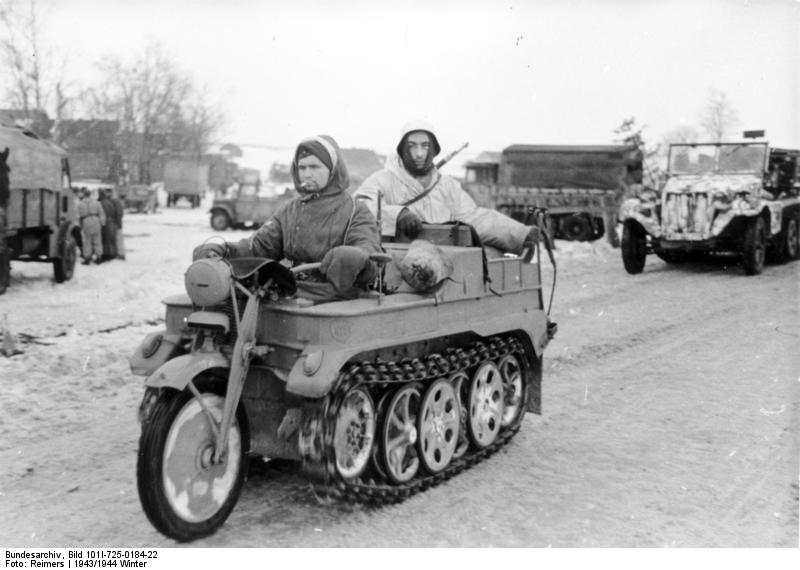
\includegraphics[width=.40\textwidth]{moto_tractora_orig.jpg}
}
\qquad
\subfigure[vehículo militar mixto]{
\label{vmm}
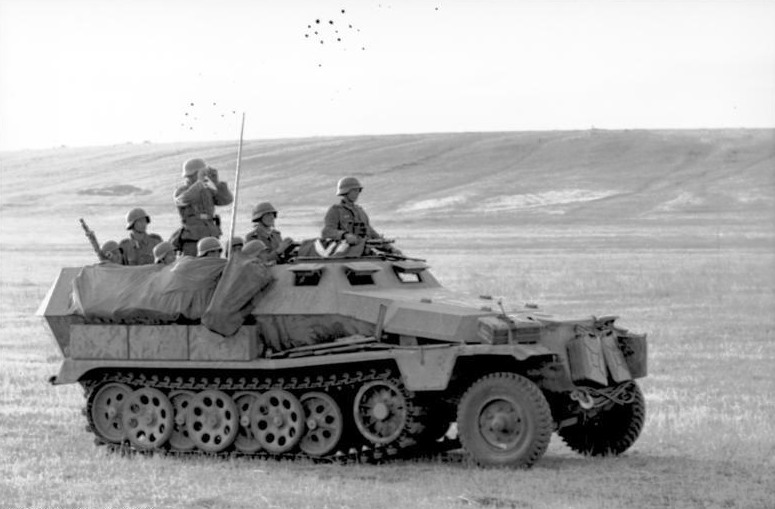
\includegraphics[width=.42\textwidth]{mixto.jpg}
}
}
\caption{\label{fig:militar} La oruga en el uso militar.}
\end{figure}

La {\it mayoría} de las \textit{orugas} forman parte de un
\emph{cinturón} flexible con un conjunto de eslabones rígidos unidos
unos a otros fuertemente. Los eslabones ayudan al vehículo a
distribuir el peso en una superficie mayor que la que hubiera tenido
con el empleo de ruedas, y esto hace que pueda moverse por un número
mayor de superficies sin hundirse debido a su propio peso. Por
ejemplo, la presión que ejerce un automóvil sobre el suelo es igual
aproximadamente a 207 kPa, mientras que las setenta toneladas que pesa
un carro M1 Abrams ejercen una presión sobre el firme de 103 kPa.

\begin{example}
  ~
  \begin{enumerate}
  \item Los tractores con una pala delante son los denominados
    bulldozers, y suelen ser usados en la construcción para remover
    tierra.
  \item Diversos vehículos incorporan la oruga en su mecánica de desplazamiento:
    \begin{enumerate}
    \item Carros de combate.
    \item Ciertos todoterreno de propósito específico, sobre todo de
      uso militar.
    \item Vehículos para el transporte por nieve e hielo.
    \end{enumerate}
  \item El transbordador espacial se transporta a su base de
    lanzamiento mediante una gran oruga transportadora.
  \item El vehículo con oruga más grande del mundo es la rotopala alemana Bagger 288.
  \end{enumerate}
\end{example}
\section{El Tractor Oruga \dots más que un 4$\mathbf{\times}$4}


Un tractor oruga es un dispositivo de transporte utilizado
principalmente en vehículos pesados, como tanques y tractores, u otro
tipo de vehículos. Consiste en un conjunto de eslabones modulares que
permiten un desplazamiento estable aún en terrenos irregulares
(cfr. \cite{bou}).

\begin{figure}[!hbp]
\centering
\mbox{
\subfigure[Rueda-piñón de un tanque Leclerc.]{
\label{hph_01}
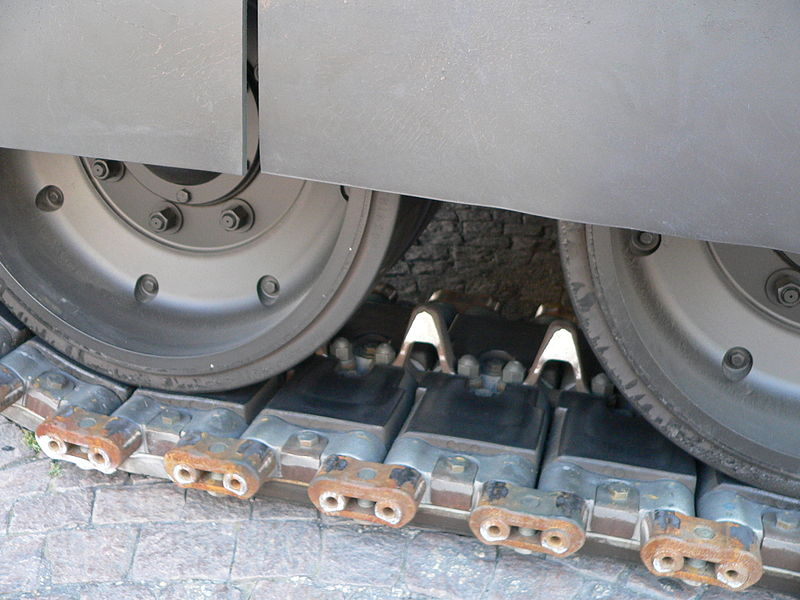
\includegraphics[width=.38\textwidth]{oruga_01.jpg}
}
\qquad
\subfigure[Rueda de rodamentos de un tanque Leclerc.]{
\label{hah}
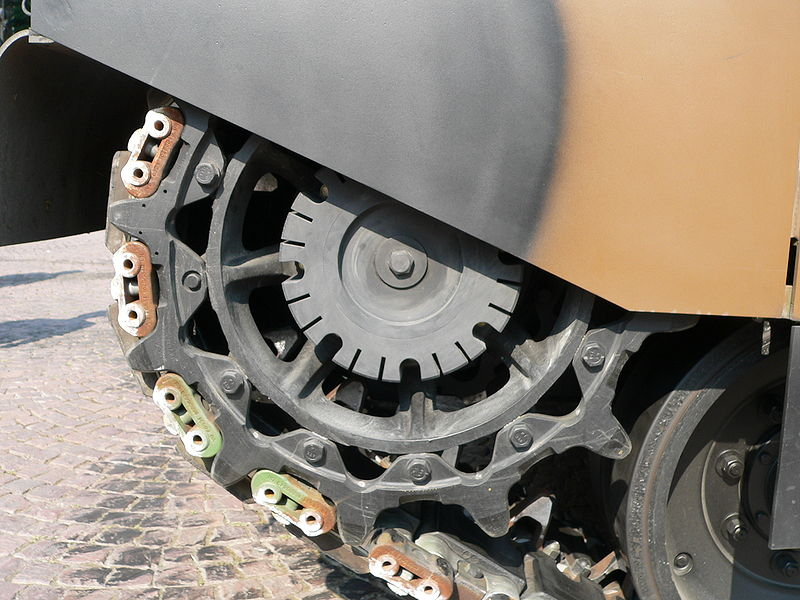
\includegraphics[width=.35\textwidth]{oruga_02.jpg}
}
}

\mbox{
\subfigure[Mi Carraro durante la carrera ]{
\label{heh}
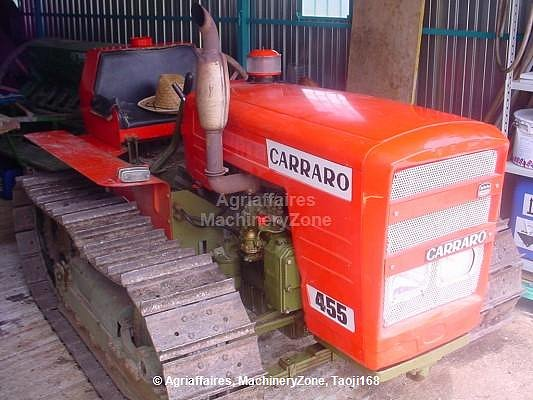
\includegraphics[width=.50\textwidth]{oruga_04.jpg}
}
}
\caption{\label{fig:oruga} Detalles de un vehículo oruga.}
\end{figure}


La cuchilla de buldózer es operado con hidráulica y esta disponible en
tres diferentes modelos: una cuchilla derecha sin ninguna curva
lateral o alas a los lados, y es usada en nivelación refinada. La
cuchilla universal es alta y curva con grandes alas laterales que le
permiten levantar un cargamento pesado. La combinación
derecha-universal cuchilla unen los dos estilos, capacidad de
retención, y curvatura, pero menos extrema en las dos. Es usada
principalmente para empujar grandes rocas amontonadas.

\section{Historia}

\subsection*{Los Orígenes}


En 1826 el ingeniero británico Sir George Cayley había patentado una
oruga mecánica con la denominación de ``universal railway'' o
ferrocarril universal. En el año 1837 el inventor ruso Dmitry
Zagryazhsky diseñó una especie de vehículo con tramos móviles y que
patentó el mismo año. Sin embargo debido a una gran falta de fondos no
pudo elaborar un prototipo. Como resultado su patente fue olvidada en
el año 1839. En 1846, el ingeniero británico James Boydell patentó una
``rueda ferroviaria sin fin''. Los tractores empujados a vapor
empleaban una forma de oruga que fue probada por la alianza occidental
durante la Guerra de Crimea en la década de 1850. Una oruga efectiva
fue inventada y construida por Alvin Lombard, que la patentó en el año
1901.



Tras el comienzo de las operaciones de Lombard, Hornsby en Inglaterra
manufacturó al menos dos vehículos ``guiados por orugas'', y su
patente fue posteriormente adquirida por Holt en 1913, permitiendo a
Holt ser popularmente conocido como el ``inventor'' de tractores
oruga. Hornsby hizo una versión para el ejército británico que
posteriormente sería la inspiración de un ``tanque''.



En la \hyperref[fig:oruga]{Figura \ref*{fig:oruga}} mostramos detalles
de la oruga de un carro de combate Leclerc (\hyperref[hph_01]{Figura
  \ref*{hph_01}} y \hyperref[hah]{Figura \ref*{hah}}) y mi medio de
vida en los duros años de exámenes e incertidumbre
(\hyperref[heh]{Figura \ref*{heh}}).

\subsection*{Tantos inventores, tantas patentes}

Las primeras semillas de la historia del tractor sobre orugas fueron
plantadas hace mas de dos siglos y medio. En 1713, Frenchman
M.D’Hermand creó un crawler tread trailer que era jalado por
cabras. En 1770, el escritor e inventor Ingles Richard Edgework
patentó el primer steam-driven moving tracking tread system. En 1826,
otro inventor Británico, llamado George Calley, desarrolló un
continuous track system que llamó la ``vía férrea universal''. En
1837, el inventor Ruso Dimitri Sagryazhsky, estuvo trabajando en un
``carruaje con orugas movibles''. Sin embargo, ninguno de estos
inventores pudo ir mas allá del papel o de la etapa del prototipo.

Alvin Lombard de Waterville Iron Works en Waterville, Maine, fue el
primero en instituir en crawler track system en la producción de
vehículos. El Lombard log hauler, patentado en 1901, fue diseñado para
mejorar la tracción en la nieve. Inicialmente, estos tractores
propulsados a vapor fueron conducidos por caballos hasta que Lombaard
instaló un steering wheel y un sled system en la parte frontal de la
máquina. Aunque los Lombard log haulers eran cazables de cargar hasta
300 toneladas, estos vehículos no fueron equipados con frenos.[3]
Ellos jalaban troncos en sleds conduciendo a una velocidad de 4 a 5
millas (6.4 a 8 Km.) por hora. En total, 83 Lombard log haulers fueron
fabricados. Con la mayoría de las ventas en Mainey y New Hampshire,
tres fueron vendidos a Rusia, uno a Wisconsin, y otro a Michigan.

A pesar del éxito inicial de Alvin Lombard, no fue hasta que el
pionero de la construcción Benjamín Holt entró en la industria del
tractor sobre orugas que la maquina se volvió realmente popular. Como
jefe de Holt Manufacturing Co. en Stockton, California, sus vehículos
sufrían por la suavidad de la rica tierra de los estados del oeste. Su
compañía empezó a experimentar con una variedad de sistemas de ruedas
para evitar que los tractores se hundieran en la tierra. Holt
Manufacturing agrego más y más ruedas hasta que sus vehículos eran 45
pies (13.7 m) de ancho, y con ruedas de 12 pies (3.7 m) de
diámetro. Holt eventualmente empezó a experimentar con tractores sobre
orugas en 1906. Lombard creyó que el tractor de Holt era una
reproducción de su log hauler y estuvo enfadado ya que Holt nunca le
pagó ningún tipo de derechos de autor. Mientras tanto, en Inglaterra,
David Roberts, el jefe de ingeniería de R. Hornsby \& Sons, patentó su
propio diseño de una oruga en 1904. Él agregó las orugas a un tractor
de aceite, pero las ventas nunca fueron tan exitosas como las de Holt
Manufacturing. Él vendió su patente a Holt en 1914.

\subsection*{El buldózer y los motores de propulsión a gas}

Holt rápidamente empezó a desarrollar motores de propulsión a gasolina
para reemplazar los tractores conducidos a vapor. En Octubre de 1906
Holt y su sobrino Pliny establecieron Aurora Engine Co. en
Stockton. En menos de dos meses estuvieron examinando su primer
motor. En 1908, las pruebas habían progresado y Holt vendió su primer
Caterpillar propulsado a gas; este fue designado el Modelo 40. Era un
motor de válvulas en cabeza con un cilindro cuádruple, 6x8 de calibre
y martillero, y clasificado en un enganche de 25 caballos de
fuerza. Inicialmente estos tractores propulsados a gas fueron
primariamente usados en proyectos agrícolas. Sin embargo, adjuntando
una grande cuchilla al frente del tractor, la utilidad de este
incremento considerablemente. Así es como el buldózer nació.

Versiones más primitivas del buldózer han sido completadas en el siglo
XIX agregando palas a los caballos, pero el tractor sobre orugas podía
incrementar su poder exponencialmente. Las primeras palas sujetadas a
los tractores tenían que ser propulsadas moviéndolas manualmente con
timones a mano. Experimentación con buldózeres mejoró al comienzo de
los años 1920s, con el primer dozer operado hidráulicamente fabricado
en 1925 por LaPlant-Choate Manufacturing Co. en Cedar Rapids,
Iowa. Esta cuchilla era enganchada al tractor en un bastidor
rectangular, pivotando en el marco del tractor sobre orugas, y
controlado por un cilindro hidráulico en la parte posterior del
tractor.

El movimiento del cuchilla fue mejorado con el desarrollo del Unidad
de Poder (PCU), introducido por Robert Gilmour Le Tourneau en 1928. La
nueva unidad era controlada por el uso de embragues y frenos, y estaba
disponible con cuatro cabrias. El unidad de poder también fue usado en
un amplio rango de otros accesorios incluyendo escrepas de jalon y
escarificadores.

Mientras que inicialmente el desarrollo del cuchilla fue realizado
separado de los tractores, compañías individuales comenzaron a unirse
con fabricantes de tractores, creando un producto más sólido y
unificado. Baker se unió con Allis-Chambers, Bucyrus-Erie se unió con
International, y Le Tourneau se unió con Caterpillar. En los años
1940s, fabricantes de tractores integraron el desarrollo de cuchillas
en sus instalaciones. Diez años después, los tractores y los cuchillas
ya no eran piezas individuales, mas bien, eran producidas para crear
un vehículo sin costuras.

\subsection*{El tractor sobre orugas durante los tiempos de guerra}

El éxito del tractor sobre orugas generó el desarrollo del tanque. Sus
orugas podían atravesar casi cualquier condición haciéndolo perfecto
para los elementos de guerra. Tuvo su primera aparición de nivel
mundial en la Primera Guerra Mundial. El desarrollo del tanque por los
Norteamericanos se quedó atrás en comparación con los Aliados Europeos
por lo que se envolvieron en la guerra bastante tarde, en 1917. Sin
embargo, después de haber presenciado el éxito de los vehículos con
orugas durante la guerra, los Estados Unidos instituyeron el
desarrollo y producción de estos vehículos en masa.

A partir de la Segunda Guerra Mundial, los tractores sobre orugas y
buldózeres habían aumentado en versatilidad. Estos fueron utilizados
en la construcción para combate en todo Europa, Asia, y el
Pacifico. Con las lodosas condiciones del terreno, no hubo otra
maquinaria que era mejor equipada para transitar el terreno que el
tractor sobre orugas. Este era responsable de mover artillería,
mientras que el buldózer nivelaba el terreno para carreteras y
aeródromos como también despejar escombros.

\section{Funcionamiento}

Las orugas están compuestas de cadena modular enlaces que forman una
cadena cerrada (cfr. \hyperref[fig:cadena]{Figura
  \ref*{fig:cadena}}). Cada enlace es amplio y frecuentemente es
fabricado con acero aleado manganeso para incrementar la resistencia y
durabilidad. La oruga esta fijada en el suelo por ruedas interiores,
llamadas bogies. Montadas en una suspensión los bogies que amortigua
el viaje. Las orugas se mueven en una rueda motriz dentada, o en una
transmisión por cadena, que se conecta a los hoyos en los enlaces de
las orugas. Además, un non-powered wheel, también conocido como ruedas
guias, es montado en un o los dos lados de las orugas para incrementar
la tensión, permitiendo que las orugas se muevan más suavemente.

\begin{figure}[!hbp]
  \centering
  \begin{minipage}{0.4\textwidth}
    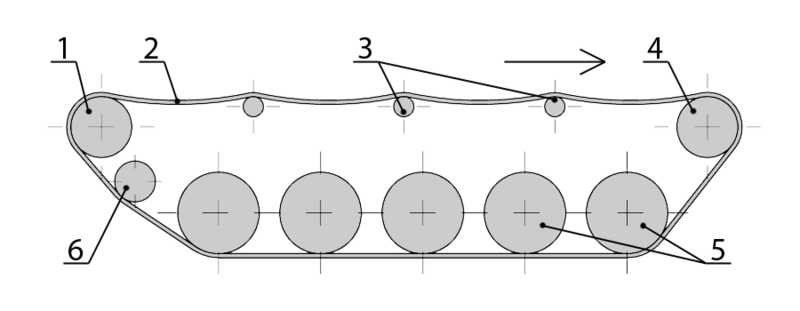
\includegraphics[width=1.5\textwidth]{oruga_03.png}
    %\caption{\label{fig:cadena_png} Esquema de la cadena}
  \end{minipage}
  \hfill
  \begin{minipage}{0.4\textwidth}
   Diagrama de una suspensión de orugas:
   \begin{enumerate}
   \item rueda de transmisión trasera
   \item oruga 
   \item rodillo de retorno
   \item rueda de transmisión delantera
   \item ruedas de rodadura
   \item rodillo tensor
   \end{enumerate}
  \end{minipage}
  \caption{\label{fig:cadena} Partes de una cadena de oruga}
\end{figure}

La cuchilla de buldózer es operado con hidráulica y esta disponible en
tres diferentes modelos: una cuchilla derecha sin ninguna curva
lateral o alas a los lados, y es usada en nivelación refinada. La
cuchilla universal es alta y curva con grandes alas laterales que le
permiten levantar un cargamento pesado. La combinación
derecha-universal cuchilla unen los dos estilos, capacidad de
retención, y curvatura, pero menos extrema en las dos. Es usada
principalmente para empujar grandes rocas amontonadas.

\nocite{let}

\section*{Referencias Web}

\begin{itemize}
\item \htmladdnormallink{Carro de combate Leclerc}
                  {http://es.wikipedia.org/wiki/AMX-56_Leclerc}

\item \htmladdnormallink{Tractores Carraro}
    {http://www.antoniocarraro.it/es}

\item \htmladdnormallink{La web de
      ritchiewiki}{http://www.es.ritchiewiki.com/wikies/index.php/Tractor_sobre_orugas}
\end{itemize}

\bibliography{oruga}

\end{document}